\appendix
\chapter{Model parameters}

\begin{table}[H]
    \centering
    \caption{\textbf{Variant 1}}
    \label{tab:variant_1}
    \renewcommand{\arraystretch}{1.3} % Adjust vertical padding
    \begin{tabular}{|c|c|c|}
        \hline
        \textbf{Parameter} & \textbf{Distribution} & \textbf{Value}\\
        \hline
        $V_{m}$ & Loguniform & (10,1000)\\
        \hline
        $K_{m}$ & Loguniform & (0.1,250)\\
        \hline
        $\mu_{m}$ & Loguniform & (0.001,50)\\
        \hline
        $D_{B}$ & Loguniform & (0.001, 10)\\
        \hline
        $D_{A}$ & Fixed & 1\\
        \hline
        $b$ & Fixed & 0.01\\
        \hline
        $n$ & Fixed & 2\\
        \hline
    \end{tabular}
\end{table}


\begin{table}[H]
    \centering
    \caption{\textbf{Variant 1 or 2}}
    \label{tab:variant_2}
    \renewcommand{\arraystretch}{1.3} % Adjust vertical padding
    \begin{tabular}{|c|c|c|}
        \hline
        \textbf{Parameter} & \textbf{Distribution} & \textbf{Value}\\
        \hline
        $V_{m}$ & Loguniform & (10,10000)\\
        \hline
        $K_{m}$ & Loguniform & (0.1,100)\\
        \hline
        $\mu_{m}$ & Loguniform & (1,100)\\
        \hline
        $D_{B}$ & Fixed & (0.01 or 10\\
        \hline
        $D_{A}$ & Fixed & (10 or 0.01)\\
        \hline
        $b$ & Loguniform & (10,10000)\\
        \hline
        $n$ & Loguniform & (2,4)\\
        \hline
    \end{tabular}
\end{table}

\chapter{Model parameters for Chapter 3}
\begin{table}
    \centering
    \begin{adjustbox}{center}
        \begin{tabular}{lllr}
            \toprule
            \textbf{Simulation ID} & \textbf{Analytical solution} & \textbf{Growth regime} & \textbf{Dr*} \\
            \midrule
             Fig.~\ref{comparison_colonies_model_vs_experiment}.1 & No steady state & T50 & 9.09 \\
             Fig.~\ref{comparison_colonies_model_vs_experiment}.2 & Turing I & T25 & 0.01 \\
             Fig.~\ref{comparison_colonies_model_vs_experiment}.3 & Turing I Unstable Stable & T25 & 0.02 \\
             Fig.~\ref{comparison_colonies_model_vs_experiment}.4 & Turing I & T50 & 0.02 \\
             Fig.~\ref{comparison_colonies_model_vs_experiment}.5 & Turing I hopf & T25 & 0.32 \\
             Fig.~\ref{comparison_colonies_model_vs_experiment}.6 & Turing I & T100 Open boundary & 0.15 \\
             Fig.~\ref{comparison_colonies_model_vs_experiment}.7 & Turning I Hopf unstable & T25 & 0.02 \\
             Fig.~\ref{comparison_colonies_model_vs_experiment}.8 & Turing I & T100 & 0.15 \\
             Fig.~\ref{system_class_simulations}.1 & Turing I Hopf & T100 & 0.10 \\
             Fig.~\ref{system_class_simulations}.2 & Turing I Hopf & T100 & 0.32 \\
             Fig.~\ref{system_class_simulations}.3 & Turing I Hopf & T100 & 0.03 \\
             Fig.~\ref{system_class_simulations}.4 & Turing I & T100 & 0.03 \\
             Fig.~\ref{system_class_simulations}.5 & Turing I & T100 & 0.01 \\
             Fig.~\ref{system_class_simulations}.6 & Turing I & T100 & 0.03 \\
             Fig.~\ref{system_class_simulations}.7 & Hopf & T50 & 0.16 \\
             Fig.~\ref{system_class_simulations}.8 & Hopf & T50 & 0.58 \\
             Fig.~\ref{system_class_simulations}.9 & Hopf & T50 & 3.69 \\
             Fig.~\ref{system_class_simulations}.10 & No steady state & T50 & 9.09 \\
             Fig.~\ref{system_class_simulations}.11 & No steady state & T50 & 64.34 \\
             Fig.~\ref{system_class_simulations}.12 & Stable Unstable Stable & T25 & 1.25 \\
             Fig.~\ref{system_class_simulations}.13 & Stable Turing Unstable & T50 & 0.01 \\
             Fig.~\ref{system_class_simulations}.14 & Stable & T25 & 25.66 \\
             Fig.~\ref{system_class_simulations}.15 & Stable & T25 & 97.13 \\
             Fig.~\ref{best_fit_colony_turing}.1 & Turing I & T50 & 0.15 \\
             Fig.~\ref{best_fit_colony_turing}.2 & Turing I Hopf & T50 & 0.10 \\
             Fig.~\ref{fig:turing_fit_noise_robustness}.4 & Turing I & T100 & 0.15 \\
             Fig.~\ref{fig:turing_fit_noise_robustness}.5 & Stable Peak near zero & T100 & 0.15 \\
             Fig.~\ref{fig:boundary_conditions_colony}.B & Turing I & T100 Open boundary & 0.15 \\
             Fig.~\ref{fig:irregular growth} & Turing I & T110 Different growth rates & 0.15 \\
            \bottomrule
        \end{tabular}
    \end{adjustbox}
    \caption{\textbf{First table of model params.} The analytical solution is derived using linear stability analysis and describes the properties of the steady-states of the system, including Turing I, Hopf, Simple stable, Simple unstable and no steady-states. The growth regimes that determine the PDE and cellular automata parameters are further specified in Table~\ref{tab:numerical_param_table}. The diffusion rate is also included.}


    \label{tab:model_param1}
\end{table}



\begin{table}
    \tiny
    \centering
    \begin{adjustbox}{center}

        \begin{tabular}{lrrrrrrrrrrrrrrrrr}
            \toprule
            \textbf{Simulation ID} & \textbf{Dr*} & \textbf{Va*} & \textbf{Vb*} & \textbf{Vc*} & \textbf{Vd*} & \textbf{Ve*} & \textbf{Vf*} & \textbf{Kub*} & \textbf{Kvd*} & \textbf{Kda*} & \textbf{Kce*} & \textbf{Kfe*} & \textbf{Keb*} & \textbf{Kee*} & \textbf{$\mu_{ASV}$} & \textbf{$\mu_{LVA}$} & \textbf{nfe} \\
            \midrule
            Fig.~\ref{comparison_colonies_model_vs_experiment}.1 & 9.09 & 74.05 & 169.38 & 669.89 & 41.12 & 39.58 & 76.52 & 15.15 & 120.03 & 1.70 & 100 & 10.73 & 5.64 & 0.01 & 3.37 & 1 & 5 \\
             Fig.~\ref{comparison_colonies_model_vs_experiment}.2 & 0.01 & 150.29 & 54.23 & 28.08 & 266.88 & 45.87 & 10.43 & 29.36 & 42.53 & 2.85 & 100.00 & 1.19 & 17.84 & 0.01 & 3.86 & 1 & 5 \\
             Fig.~\ref{comparison_colonies_model_vs_experiment}.3 & 0.02 & 795.88 & 29.76 & 14.26 & 21.69 & 19.04 & 48.66 & 150.98 & 6.42 & 1.46 & 100.00 & 15.15 & 11.34 & 0.01 & 4.46 & 1 & 5 \\
             Fig.~\ref{comparison_colonies_model_vs_experiment}.4 & 0.02 & 45.20 & 603.17 & 234.59 & 158.98 & 70.72 & 13.73 & 13.93 & 239.29 & 1.97 & 100.00 & 2.35 & 60.56 & 0.01 & 3.99 & 1 & 5 \\
             Fig.~\ref{comparison_colonies_model_vs_experiment}.5 & 0.32 & 48.36 & 786.32 & 31.16 & 264.07 & 30.32 & 164.65 & 14.38 & 251.50 & 7.89 & 100 & 28.85 & 28.75 & 0.01 & 3.83 & 1 & 5 \\
             Fig.~\ref{comparison_colonies_model_vs_experiment}.6 & 0.15 & 21.67 & 321.54 & 16.88 & 5.29 & 8.60 & 3.57 & 43.93 & 26.33 & 0.73 & 2.34 & 1.41 & 1.53 & 0.001 & 3.57 & 1 & 8 \\
             Fig.~\ref{comparison_colonies_model_vs_experiment}.7 & 0.02 & 113.58 & 725.58 & 322.38 & 240.91 & 21.66 & 13.29 & 80.20 & 10.45 & 24.96 & 100.00 & 7.56 & 4.46 & 0.01 & 3.53 & 1 & 5 \\
             Fig.~\ref{comparison_colonies_model_vs_experiment}.8 & 0.15 & 21.67 & 321.54 & 16.88 & 5.29 & 8.60 & 3.57 & 43.93 & 26.33 & 0.73 & 2.34 & 1.41 & 1.53 & 0.001 & 3.57 & 1 & 8 \\
             Fig.~\ref{system_class_simulations}.1 & 0.10 & 495.68 & 872.38 & 697.87 & 372.08 & 109.70 & 14.56 & 53.14 & 219.76 & 4.99 & 100.00 & 2.75 & 77.39 & 0.01 & 3.70 & 1 & 5 \\
             Fig.~\ref{system_class_simulations}.2 & 0.32 & 48.36 & 786.32 & 31.16 & 264.07 & 30.32 & 164.65 & 14.38 & 251.50 & 7.89 & 100.00 & 28.85 & 28.75 & 0.01 & 3.83 & 1 & 5 \\
             Fig.~\ref{system_class_simulations}.3 & 0.03 & 301.23 & 83.90 & 491.96 & 868.92 & 131.53 & 63.43 & 133.37 & 68.45 & 9.85 & 100.00 & 3.09 & 73.83 & 0.01 & 3.70 & 1 & 5 \\
             Fig.~\ref{system_class_simulations}.4 & 0.03 & 193.50 & 22.54 & 626.85 & 106.80 & 402.97 & 39.13 & 13.91 & 4.82 & 6.61 & 100.00 & 23.70 & 336.49 & 0.01 & 3.18 & 1 & 5 \\
             Fig.~\ref{system_class_simulations}.5 & 0.01 & 19.53 & 12.34 & 123.40 & 51.73 & 40.95 & 91.98 & 7.07 & 2.98 & 6.18 & 100.00 & 50.56 & 32.69 & 0.01 & 4.56 & 1 & 5 \\
             Fig.~\ref{system_class_simulations}.6 & 0.03 & 816.37 & 77.89 & 58.00 & 63.95 & 59.97 & 12.78 & 110.34 & 49.06 & 3.22 & 100.00 & 3.38 & 50.31 & 0.01 & 3.49 & 1 & 5 \\
             Fig.~\ref{system_class_simulations}.7 & 0.16 & 11.99 & 82.80 & 517.54 & 118.80 & 12.02 & 500.10 & 4.90 & 16.60 & 22.21 & 100.00 & 372.67 & 2.19 & 0.01 & 3.59 & 1 & 5 \\
             Fig.~\ref{system_class_simulations}.8 & 0.58 & 311.01 & 452.00 & 609.80 & 140.64 & 511.01 & 264.43 & 267.90 & 23.40 & 17.44 & 100.00 & 80.26 & 10.13 & 0.01 & 3.86 & 1 & 5 \\
             Fig.~\ref{system_class_simulations}.9 & 3.69 & 138.98 & 718.76 & 731.67 & 574.33 & 893.73 & 274.09 & 45.83 & 231.33 & 3.65 & 100.00 & 127.68 & 5.88 & 0.01 & 3.82 & 1 & 5 \\
             Fig.~\ref{system_class_simulations}.10 & 9.09 & 74.05 & 169.38 & 669.89 & 41.12 & 39.58 & 76.52 & 15.15 & 120.03 & 1.70 & 100.00 & 10.73 & 5.64 & 0.01 & 3.37 & 1 & 5 \\
             Fig.~\ref{system_class_simulations}.11 & 64.34 & 229.84 & 199.15 & 822.04 & 58.37 & 137.50 & 18.27 & 9.68 & 70.64 & 2.17 & 100.00 & 8.96 & 23.36 & 0.01 & 3.26 & 1 & 5 \\
             Fig.~\ref{system_class_simulations}.12 & 1.25 & 11.76 & 134.85 & 286.24 & 168.35 & 306.73 & 398.68 & 3.15 & 15.85 & 160.35 & 100.00 & 84.35 & 1.32 & 0.01 & 3.13 & 1 & 5 \\
             Fig.~\ref{system_class_simulations}.13 & 0.01 & 165.48 & 100.21 & 52.73 & 377.51 & 192.76 & 603.27 & 70.15 & 12.06 & 127.57 & 100 & 131.70 & 1.66 & 0.01 & 4.45 & 1 & 5 \\
             Fig.~\ref{system_class_simulations}.14 & 25.66 & 825.22 & 30.51 & 130.99 & 30.67 & 166.25 & 630.74 & 238.35 & 4.73 & 13.41 & 100.00 & 1.85 & 147.94 & 0.01 & 3.16 & 1 & 5 \\
             Fig.~\ref{system_class_simulations}.15 & 97.13 & 259.08 & 179.44 & 127.45 & 674.32 & 19.68 & 14.12 & 76.32 & 3.39 & 392.99 & 100.00 & 1.28 & 14.09 & 0.01 & 2.81 & 1 & 5 \\
             Fig.~\ref{best_fit_colony_turing}.1 & 0.15 & 21.74 & 321.61 & 16.95 & 5.27 & 8.54 & 3.57 & 0.15 & 26.39 & 16.95 & 5.27 & 1.42 & 1.52 & 0.001 & 3.60 & 1 & 8 \\
             Fig.~\ref{best_fit_colony_turing}.2 & 0.10 & 102.69 & 431.77 & 25.23 & 7.44 & 4.90 & 3.61 & 0.10 & 29.99 & 25.23 & 7.44 & 1.58 & 0.79 & 0.001 & 3.69 & 1 & 8 \\
             Fig.~\ref{fig:turing_fit_noise_robustness}.4 & 0.15 & 21.67 & 321.54 & 16.88 & 5.29 & 8.60 & 3.57 & 43.93 & 26.33 & 0.73 & 2.34 & 1.41 & 1.53 & 0.001 & 3.57 & 1 & 8 \\
             Fig.~\ref{fig:turing_fit_noise_robustness}.5 & 0.15 & 21.94 & 327.41 & 16.71 & 5.30 & 8.55 & 3.58 & 44.06 & 26.51 & 0.72 & 2.31 & 1.41 & 1.53 & 0.001 & 3.62 & 1 & 8 \\
             Fig.~\ref{fig:boundary_conditions_colony}.B & 0.15 & 21.67 & 321.54 & 16.88 & 5.29 & 8.60 & 3.57 & 43.93 & 26.33 & 0.73 & 2.34 & 1.41 & 1.53 & 0.001 & 3.57 & 1 & 8 \\
             Fig.~\ref{fig:irregular growth} & 0.15 & 21.67 & 321.54 & 16.88 & 5.29 & 8.60 & 3.57 & 43.93 & 26.33 & 0.73 & 2.34 & 1.41 & 1.53 & 0.001 & 3.57 & 1 & 8 \\
            \bottomrule
        \end{tabular}
    \end{adjustbox}
    \caption{\textbf{Second table of model params.} The kinetic parameters for the dimensionless model are listed here. $\mu_{ASV}$ corresponds to $\mu_{A}$ while $\mu_{LVA}$ corresponds to $\mu_{B}$, $\mu_{C}$, $\mu_{D}$, $\mu_{E}$, $\mu_{F}$. Cooperativity rates are not shown in this table but fixed to $n_{ub}=1$, $n_{ee}=4$, $n_{eb}=4$, $n_{vd}=2$, $n_{da}=2$ and $n_{ce}=3$. }

    \label{tab:model_param2}
\end{table}




\chapter{Growth regimes in cellular automata model}\label{appendix_growth_rates}
\begin{figure}[H] % h! is a placement specifier; it tries to place the image here.
    \centering
    \begin{adjustbox}{center}
        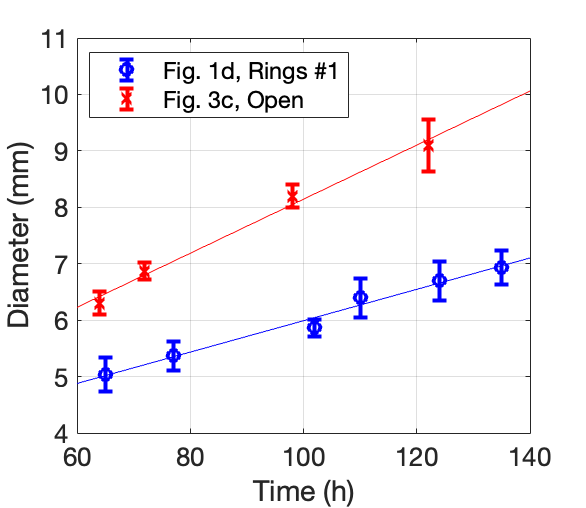
\includegraphics[width=0.6\textwidth]{chapters/Appendix/fig_growth_curves_e20210611} % The name of your image file; assumes it is in the same directory as your .tex file
    \end{adjustbox}
    \caption{\textbf{Growth rate of two experimental colonies.} Figure produced by Dr. Jure Tica. Image processing software was used to measure the size of the colony diameter across two different axes, this variability is captured in the error bars (± SEM, n = 2). Two colonies that grow equally in all directions (isotropic growth) were used as examples.}
    \label{fig:fig_growth_curves_e20210611}
\end{figure}

\begin{figure}[H] % h! is a placement specifier; it tries to place the image here.
    \centering
    \begin{adjustbox}{center}
        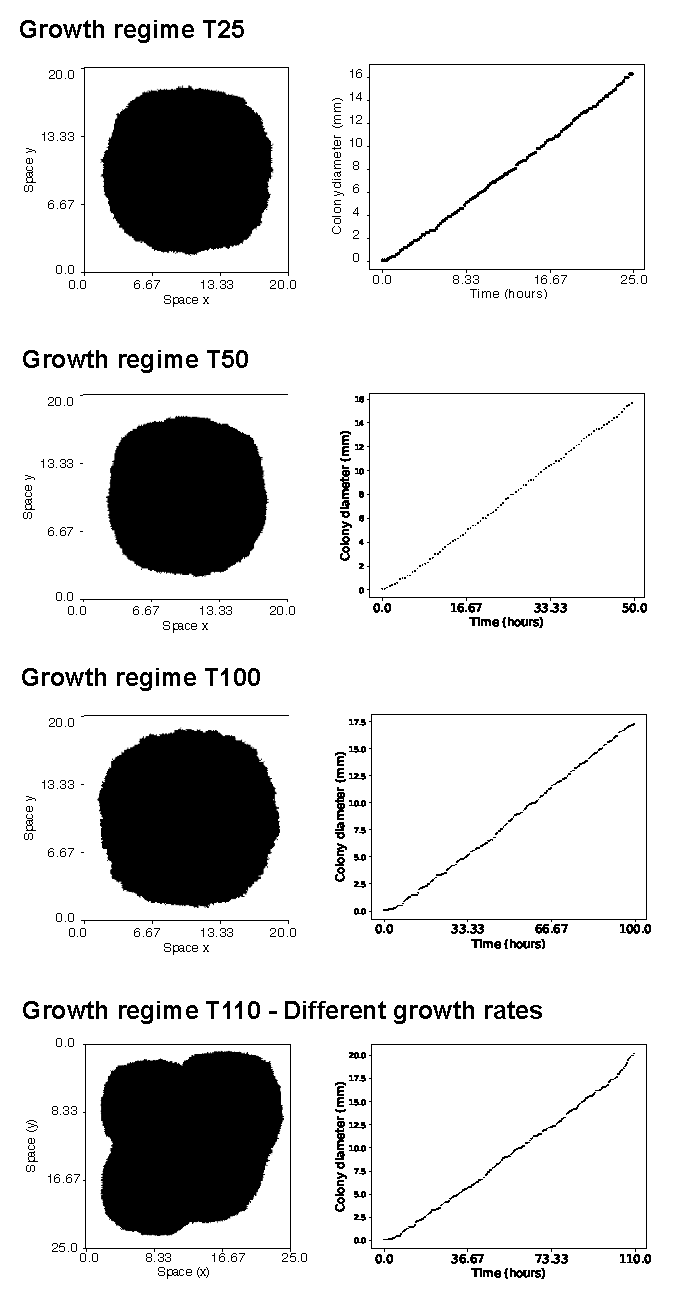
\includegraphics[width=0.8\textwidth]{chapters/Appendix/ca_growth_regimes} % The name of your image file; assumes it is in the same directory as your .tex file
    \end{adjustbox}
    \caption{\textbf{Bacterial colony and growth curves from cellular automata simulations.} Using different growth regimes (left) final snapshot of bacterial colony and (right) growth curve of bacterial colony. Dimensionless time and space is shown here. }
    \label{fig:ca_growth_regimes}
\end{figure}


\begin{table}[H]
    \centering
    \begin{adjustbox}{center}

        \begin{tabular}{lrrrrrrrlrrl}
        \toprule
        \textbf{Growth regime} & \textbf{L} & \textbf{T} & \textbf{J} & \textbf{N} & \textbf{dx} & \textbf{dt} & \textbf{Boundary}  & \textbf{Random seed} & \textbf{m} & \textbf{$p_{d}$} \\
        \midrule
        T10 & 20 & 10 & 200 & 500 & 0.1 & 0.02 & 1  & 1 & 0.2 & 0.7 \\
        T25 & 20 & 25 & 200 & 1250 & 0.1 & 0.02 & 1  & 1 & 0.2 & 0.7 \\
        T50 & 20 & 50 & 200 & 2500 & 0.1 & 0.02 & 1  & 1 & 0.5 & 1 \\
        T50 Open boundary & 20 & 50 & 200 & 2500 & 0.1 & 0.02 & 2  & 1 & 0.5 & 1 \\
        T100 & 20 & 100 & 200 & 5000 & 0.1 & 0.02 & 1  & 1 & 0.5 & 0.38 \\
        T110 Different growth rates & 25 & 110 & 250 & 5500 & 0.1 & 0.02 & 1 & 1 & 0.5 & 0.38 and 0.91 \\
        \bottomrule
    \end{tabular}
        \end{adjustbox}

    \caption{Cellular automata and PDE solver parameters for different growth regimes.}
    \label{tab:numerical_param_table}
\end{table}


